\section{Teilbarkeit}

Sei $R$ ein \textbf{nullteilfreier} Ring.

\begin{definition}[teilt, assoziert, irreduzibel, prim, ggT, kgV]
	\proplbl{2_4_1}
	Seinen $x,y,z,p \in R$.
	\begin{enumerate}[label=(\alph*)]
		\item $x$ \begriff{teilt} $y$ (in Zeichen $x \mid y$) $\Leftrightarrow \exists z \in R: xz = y$
		\item $x$ ist \begriff{assoziert} zu $y$ (in Zeichen $x \sim y$) $\Leftrightarrow \exists z \in R^{\times}, xz = y$
		\item $p$ ist \begriff{irreduzibel} $\Leftrightarrow p \not \in R^{\times} \cup \{  0\}$ und $\forall x,y \in R$:
		\begin{align}
			p = xy &\Rightarrow x \in R^{\times} \text{ oder } y \in R^{\times} \notag
		\end{align}
		\item $p$ ist \begriff{prim} $\Leftrightarrow  p \not \in R^{\times} \cup \{ 0 \}$ und $\forall x,y \in R$:
		\begin{align}
			p \mid xy &\Rightarrow p \mid x \text{ oder } p \mid y \notag
		\end{align}
		\item $z$ ist \begriff{größter gemeinsamer Teiler} von $x,y$ (in Zeichen $z = \ggT(x,y)$) $\Leftrightarrow  z \mid x$ und $z \mid y$ und $\forall a \in R: a\mid x$ und $a \mid y\Rightarrow a \mid z$
		\item $z$ ist \begriff{kleinstes gemeinsames Vielfaches} von $x,y$ (in Zeichen $z = \kgV(x,y)$) $\Leftrightarrow x \mid z$ und $y \mid z$ und $\forall a \in R: x \mid a$ und $y \mid a \Rightarrow z \mid a$
	\end{enumerate}
\end{definition}

\begin{remark}
	\begin{enumerate}[label=(\alph*)]
		\item $x \mid y \Leftrightarrow y \in (x) \Leftrightarrow (y) \subseteq (x)$
		\item $x \sim y \Leftrightarrow x \mid y \text{ und } y \mid x \Leftrightarrow (x) = (y)$
		\item $p$ prim $\Leftrightarrow (p)$ prim und $p \neq 0$
		\item $p$ prim $\Rightarrow p$ irreduzibel
		\item Analog zu e) und f) in \propref{2_4_1} kann man ein $\ggT$ bzw. $\kgV$ von endlich vielen Elementen von $R$ definieren.
	\end{enumerate}
\end{remark}
\begin{proof}
	\begin{itemize}
		\item[d)] $p = xy \Rightarrow p \mid xy \xRightarrow{p \text{ prim}} p \mid x \text{ oder } p\mid y$, ohne Einschränkung $p \mid x$, das heißt $x = px'$ mit $x' \in R \Rightarrow p(1-x'y) =0 \Rightarrow 1 - x'y = 0 \Rightarrow 1 = x'y \Rightarrow y \in R^{\times}$
	\end{itemize}
\end{proof}

\begin{definition}[euklidisch, Hauptidealring, faktoriell]
	\begin{enumerate}[label=(\alph*)]
		\item $R$ ist \begriff{euklidisch} $\Leftrightarrow$ es gibt eine euklidische Gradfunktion:
		\begin{align}
			\delta: R\setminus \{0\} \to \natur_0 \notag
		\end{align}
		mit $\forall x,y \in R\setminus \{0\} \exists q,r \in R$ mit $x = qy + r$ und $r=0$ oder $\delta(r) < \delta(y)$
		\item $R$ ist \begriff{Hauptidelring} $\Leftrightarrow$ Jedes Ideal $I \unlhd R$ ist ein Hauptideal.
		\item $R$ ist \begriff{faktoriell} $\Leftrightarrow$ Jedes $0 \neq x \in R\setminus R^{\times}$ ist ein Produkt von Primelementen.
	\end{enumerate}
\end{definition}

\begin{proposition}
	$R$ euklidisch $\Rightarrow R$ Hauptidealring $\Rightarrow R$ faktoriell.
\end{proposition}

\begin{proof}
	LAAG VIII.3.6 und VIII.4.4.
\end{proof}

\begin{example}
	\begin{enumerate}[label=(\alph*)]
		\item $\whole$, $K[x]$: euklidisch
		\item $K$ Körper: euklidisch
		\item $\whole[i] = \{ a+b\sqrt{-1} \mid a,b \in \whole \} \subseteq \comp$: euklidisch mit $\delta(z) = \vert z \vert^2$
		\item $K[x,y], \whole[x]$: keine Hauptidealringe
		\item $\whole[\sqrt{-5}] = \{ a+b\sqrt{-5} \mid a,b \in \whole \} \subseteq \comp$: nicht faktoriell, da $6 = 2\cdot 3 = (1 + \sqrt{-5})(1-\sqrt{-5})$
	\end{enumerate}
\end{example}

\begin{remark}
	Ist $R$ faktoriell, so gilt:
	\begin{enumerate}[label=(\alph*)]
		\item $p$ irreduzibel $\Leftrightarrow p$ prim
		\item Eine Darstellung von $0 \neq x \in R \setminus R^{\times}$ als Produkt von Primelementen ist eindeutig bis auf Reihenfolge und Assoziiertheit.
	\end{enumerate}
\end{remark}

\begin{proposition}
	Sei $R$ ein Hauptidealring. Wenn $(0) \neq \mathfrak{p} \unlhd R$ ein Primideal ist, so ist $\mathfrak{p}$ maximal.
\end{proposition}

\begin{proof}
	Sei $\mathfrak{p} \subseteq I \unlhd R$. Da $R$ ein Hauptidealring ist, kann man $\mathfrak{p} = (p)$ mit $p \in R$ prim schreiben. $p$ ist prim, insbesondere irreduzibel. Weiterhin gilt $I = (a)$ mit $a \in R$ und $a \mid p$. Da $p$ prim, gilt $a \sim 1$ oder $a \sim p$. Also $I = R$ oder $I = \mathfrak{p}$. Damit ist $\mathfrak{p}$ maximal.
\end{proof}

\begin{remark}
	In jedem Hauptidealring gilt:
	\begin{align}
		(x) + (y) = (\ggT(x,y)) \notag
	\end{align}
	anders gesagt
	\begin{align}
		\ggT(x,y) = ax + by \notag
	\end{align}
	mit $a,b \in R$. In euklidischen Ringen können $a$ und $b$ explizit bestimmt werden.
\end{remark}

\begin{proposition}[Erweiterter euklidischer Algorithmus]
	Sei $R$ euklidisch mit euklidischer Gradfunktion $\delta$, und seien $x,y \in R$. Man setze $x_0 = x$, $x_1 = y$, $a_0=1$ $b_0 = 0$, $a_1 = 0$, $b_1 = 1$ und berechne iterativ $x_{i+1}$, $q_{i+1}$, $a_{i+1}$, $b_{i+1}$ für $i \ge 1$ als
	\begin{align}
		x_{i-1} &= q_{i+1}x_i + x_{i+1} &\qquad &x_{i+1} = 0 \text{ oder } \delta(x_{i+1}) < \delta(x_i) \notag \\
		a_{i+1} &= a_{i-1} + q_{i+1}a_i & & \notag \\
		b_{i+1} &= b_{i-1} - q_{i+1}b_i & & \notag
	\end{align}
	solange bis $x_{k+1} = 0$. Dann ist
	\begin{align}
		\ggT(x,y) = x_k = a_k x + b_k y \notag
	\end{align}
\end{proposition}

\begin{proof}
	Da $\delta(x_1) > \delta(x_2) > \dots$ wird $x_{k+1} = 0$ irgendwann erreicht. Für jedes $i \le k$ ist 
	\begin{align}
		\ggT(x_{i-1}, x_i) &= \ggT(q_{i+1}x_i + x_{i+1}, x_i)\notag \\
		&=\ggT(x_{i+1}, x_i) \notag \\
		&= \ggT(x_i, x_{i+1}) \notag
	\end{align}
	somit im Allgemeinen:
	\begin{align}
		\ggT(x,y) &= \ggT(x_0,x_1) = \dots = \ggT(x_k, \underbrace{x_{k+1}}_{=0}) = x_k \notag
	\end{align}
	Per Induktion sieht man, dass $x_i = a_i x + b_i y$ für alle $i \le k: x_{i-1} = a_{i-1} x + b_{i-1}y$, $x_i = a_i x + b_i y$ sowie $x_{i-1} = q_{i+1} x_i + x_{i+1}$\\
	\begin{align}
	\Rightarrow x_{i+1} &= x_{i-1}q_{i+1}x_i = (a_{i+1} - q_{i+1} a_i)x + (b_{i-1}-q_{i+1}b_i)y \notag\\
	&= a_{i+1}x + b_{i+1}y\notag
	\end{align}
\end{proof}

\begin{example}
	$R = \whole$, $x = \textcolor{red}{5}$, $y= \textcolor{blue}{13}$
	\begin{center}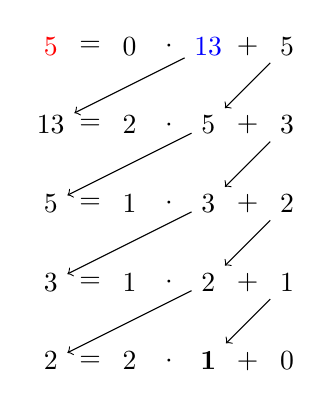
\begin{tikzpicture}
		\node at (0,0) (gleich) {$=$};
		\node at (0,-1) (gleich) {$=$};
		\node at (0,-2) (gleich) {$=$};
		\node at (0,-3) (gleich) {$=$};
		\node at (0,-4) (gleich) {$=$};
		
		\node at (1,0) (mal) {$\cdot$};
		\node at (1,-1) (mal) {$\cdot$};
		\node at (1,-2) (mal) {$\cdot$};
		\node at (1,-3) (mal) {$\cdot$};
		\node at (1,-4) (mal) {$\cdot$};
		
		\node at (2,0) (plus) {$+$};
		\node at (2,-1) (plus) {$+$};
		\node at (2,-2) (plus) {$+$};
		\node at (2,-3) (plus) {$+$};
		\node at (2,-4) (plus) {$+$};
		
		\node[red] at (-0.5,0) (erg1) {5};
		\node at (-0.5,-1) (erg2) {13};
		\node at (-0.5,-2) (erg3) {5};
		\node at (-0.5,-3) (erg4) {3};
		\node at (-0.5,-4) (erg5) {2};
		
		\node at (0.5,0) (fak1) {0};
		\node at (0.5,-1) (fak2) {2};
		\node at (0.5,-2) (fak3) {1};
		\node at (0.5,-3) (fak4) {1};
		\node at (0.5,-4) (fak5) {2};
		
		\node[blue] at (1.5,0) (quot1) {13};
		\node at (1.5,-1) (quot2) {5};
		\node at (1.5,-2) (quot3) {3};
		\node at (1.5,-3) (quot4) {2};
		\node at (1.5,-4) (quot5) {\textbf{1}};
		
		\node at (2.5,0) (plus1) {5};
		\node at (2.5,-1) (plus2) {3};
		\node at (2.5,-2) (plus3) {2};
		\node at (2.5,-3) (plus4) {1};
		\node at (2.5,-4) (plus5) {0};
		
		\draw[->] (quot1) -- (erg2);
		\draw[->] (quot2) -- (erg3);
		\draw[->] (quot3) -- (erg4);
		\draw[->] (quot4) -- (erg5);
		
		\draw[->] (plus1) -- (quot2);
		\draw[->] (plus2) -- (quot3);
		\draw[->] (plus3) -- (quot4);
		\draw[->] (plus4) -- (quot5);
		\end{tikzpicture}\end{center}
	$\Rightarrow \ggT(5,13) = 1 = 2\cdot 13 - 5 \cdot 5$
\end{example}

\begin{example}
	Bestimme $x \in \whole$ mit $x \equiv 1 \mod 5$ und $x \equiv 2 \mod 13$.\\
	$b_1 = 2 \cdot 13 = 26$
	\begin{align}
		b_1 &\equiv 1 \mod 5 \notag \\
		b_1 &\equiv 0 \mod 13\notag 
	\end{align}
	$b_2 = -5\cdot 5 = -25$
	\begin{align}
		b_2 &\equiv 0 \mod 5\notag \\
		b_2 &\equiv 1 \mod 13\notag
	\end{align}
	Setze $x = 1\cdot b_1 + 2 \cdot b_2 = -24$. Die anderen sind $x+5\cdot 13\whole=41+65\whole$.
\end{example}